\subsection{アプリケーションの開発環境}
 webアプリケーション開発にはjavascriptのwebフレームワークであるNode.jsを用いた.Node.jsのパッケージであるexpressとnanoを用いた.expressはwebフレームワークで、nanoはCouchDBのためのドライバである.

\begin{table}[htb]
	\begin{tabular}{|l|c|r|r|}\hline
	導入ソフト & ヴァージョン \\ \hline \hline
	Node.js & 0.12.6 \\ \hline
	Express & 4.12.1 \\ \hline
	Passport & 未定 \\ \hline
	\end{tabular}
\end{table}


\subsection{データベースの設計}
	CouchDBにss-mixの仕様書から引っ張ってきたデータ格納方法およびデータ定義\cite{bibi1}に基づいてデータを格納する.CouchDBはひとつのデータベースの中に複数のドキュメントとよばれるデータ構造を保持している.このドキュメントは事前にテーブルなどで定義する必要がない.

	本研究ではひとつの医療行為に対してひとつのドキュメントで管理する.ドキュメントが保持する情報を\ref{tab:doc}に示す.


\begin{table}[htb]
	\caption{ドキュメントが保持する情報}
	\begin{tabular}{|l|c|r|r|}\hline
	Key & Value \\ \hline \hline
	id &  患者名、日付、その日に追加された順番がidとなる.\\
				ドキュメントを一意に定めるためのID.\\
				デフォルトではCouchDBによって自動で割り振られる.\\ \hline
	rev & ドキュメントの更新回数を示す. 更新時に参照し競合を防ぐ. \\ \hline
	name & 患者の名前 \\ \hline
	data & 医療行為によって得られた情報をjsonで格納. \\ \hline
	\end{tabular}
	\label{tab:doc}
\end{table}



	\begin{figure}[htbp]
		\begin{center}
			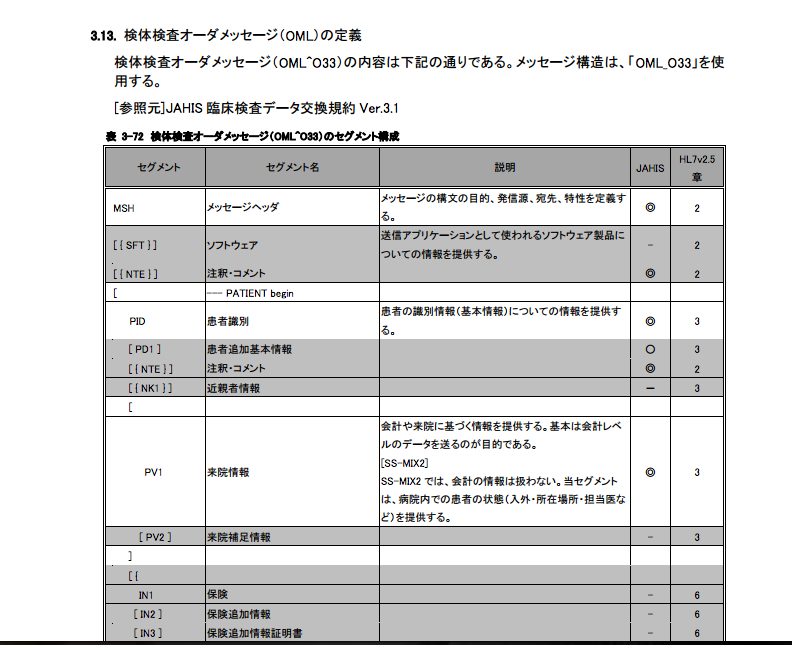
\includegraphics[width=5cm, bb=0 0 645 790]{./gazou/ss-mix_sample.png} %よこたて
		\end{center}
		\caption{データ定義}
		\label{ss-mix_sample}
	\end{figure}

	\begin{figure}[htbp]
		\begin{center}
			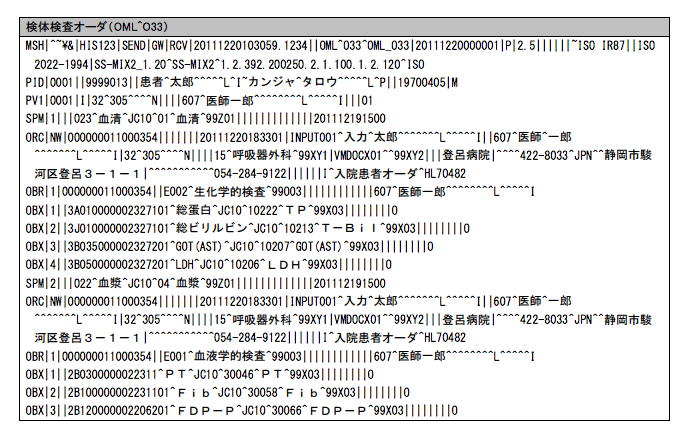
\includegraphics[width=5cm, bb=0 0 437 688]{ss-mix_sampledata.png}
		\end{center}
		\caption{データサンプル}
		\label{ss-mix_sampledata}
	\end{figure}

\subsection{アプリケーションの設計}

	\subsubsection{新出のフォーマットのドキュメントに対するコスト}
	縦向き、横向きのcsv(地域の病院で生まれるような電子化された医療情報)はノーコスト.
	電子カルテ固有の出力ファイルはHL7に対応していればノーコスト.
	json型にもってくまでができれば入力できる.
	出力にはkeyを関連付けるためのコストがかかるが,これは利用者がチューニングしていく.


\subsection{アプリケーションの機能}
 医療情報を収集するNoSQLデータベースシステム.UIとしてWebアプリを用意し、医療関係者、薬剤師、患者の3者に対して、情報を扱いやすいようにした.

	\subsubsection{患者情報閲覧}
		getdb
		\\
		\begin{figure}[htbp]
			%\begin{center}
				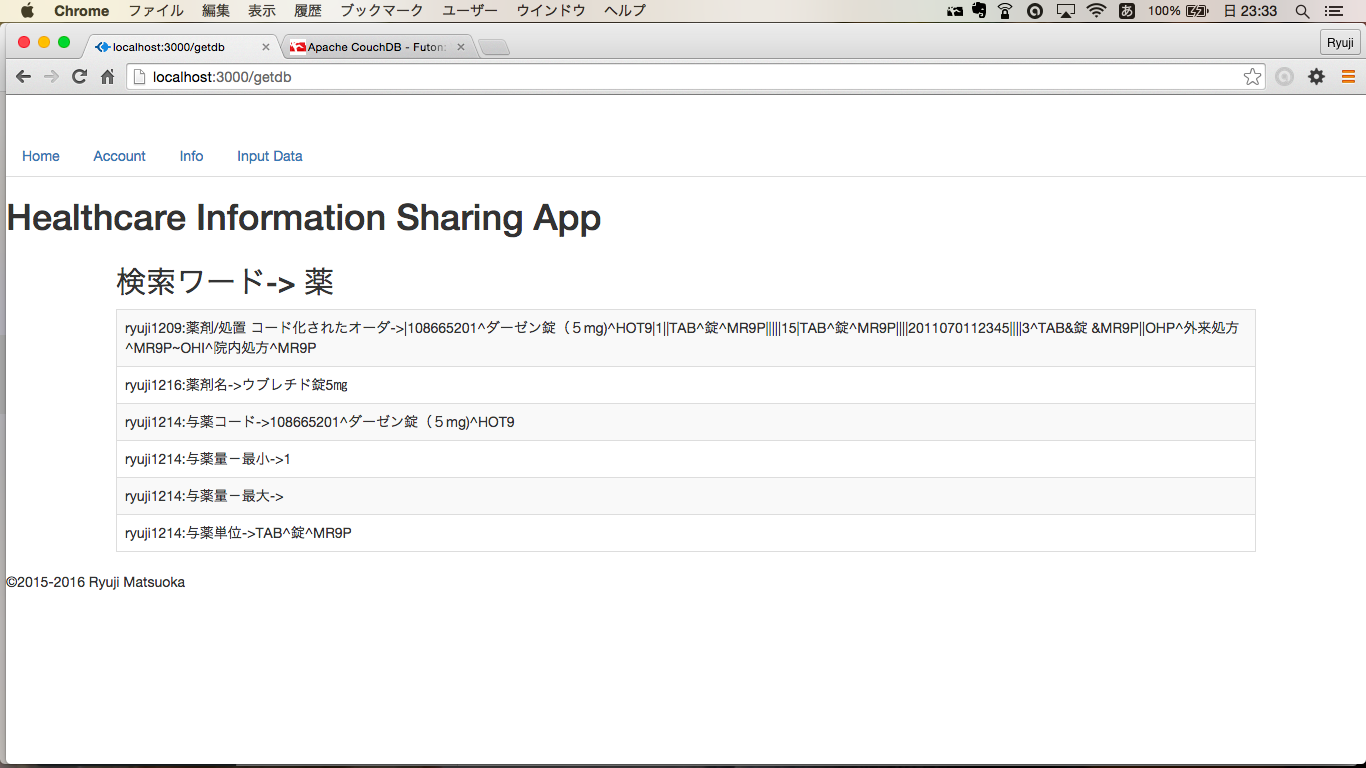
\includegraphics[width=5cm, bb=0 0 437 688]{./gazou/getdb.png}
			%\end{center}
			\caption{薬 でデータ抽出した様子}
			\label{ss-mix_sampledata}
		\end{figure}
		正規表現によって検索ワードを元に必要な情報を抜き出す
		必要な人に必要な情報が見えるヴューを用意する.
		血圧とか、血糖とか、項目を指定したらその項目の数値を
		異なるフォーマットによって投入されてるドキュメントからひっぱってきて表示する.

	%\subsubsection{共有の許可,権限}
	%	患者が情報共有する医療関係者を選択する.


\subsection{データの投入方法}

	\begin{figure}[htbp]
		\begin{center}
			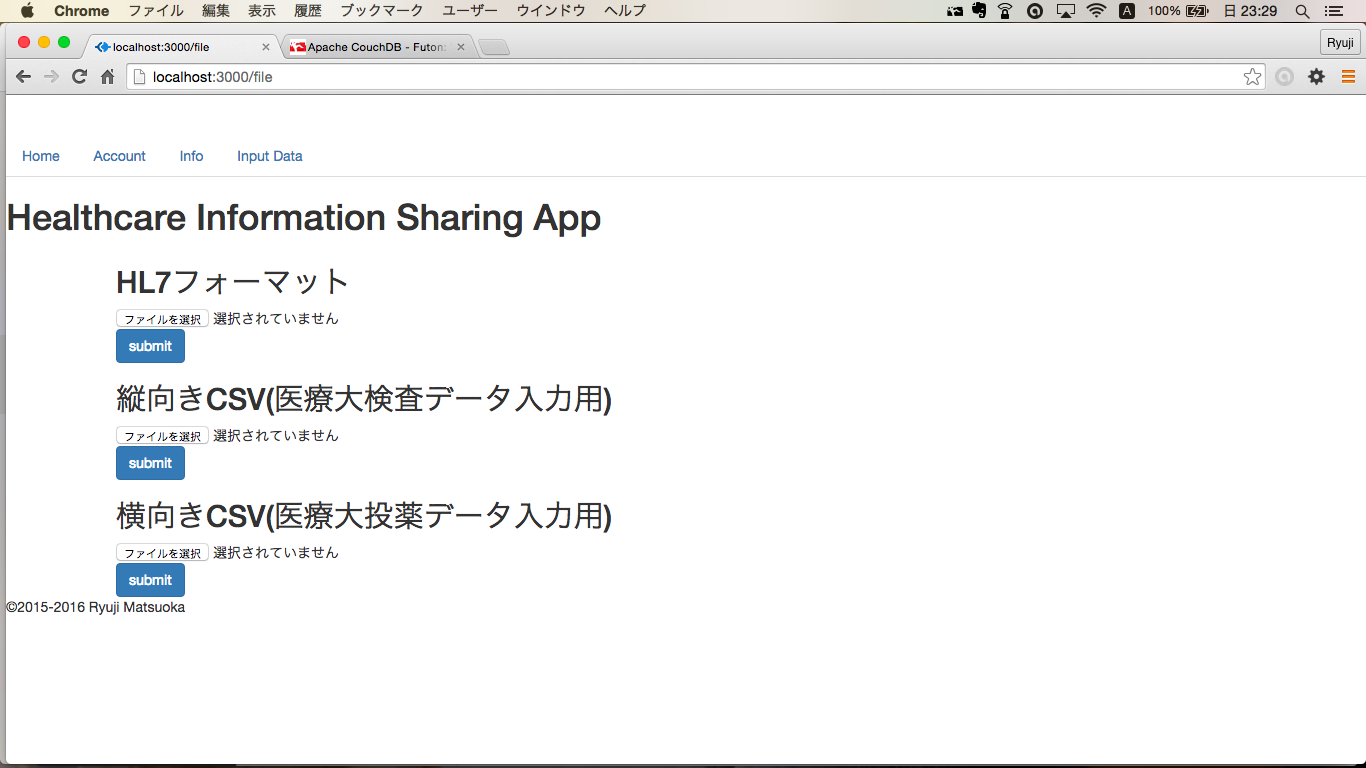
\includegraphics[width=5cm, bb=0 0 437 688]{./gazou/fileiopage.png}
		\end{center}
		\caption{ファイル入力ページ}
		\label{ss-mix_sampledata}
	\end{figure}

	dbaccess
	1診療1ドキュメント
	どうやってCouchからデータを引っ張ってきているか.
	患者のドキュメントを検索してからデータを取得.
		\subsubsection{縦向きcsvファイルの場合}
			parse
			医療大の検査データ
			\\
			\begin{figure}[htbp]
				%\begin{center}
					%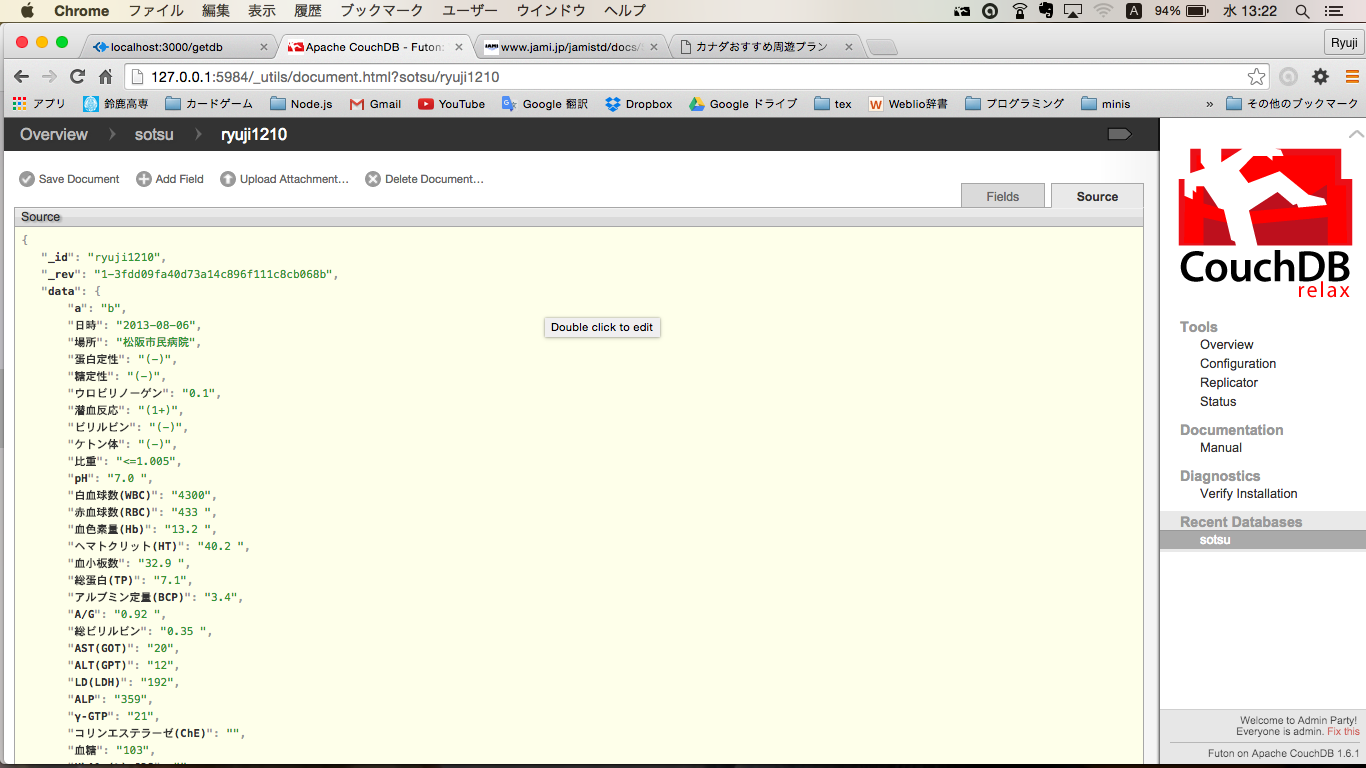
\includegraphics[width=5cm, bb=0 0 437 688]{./gazou/kensa.png}
					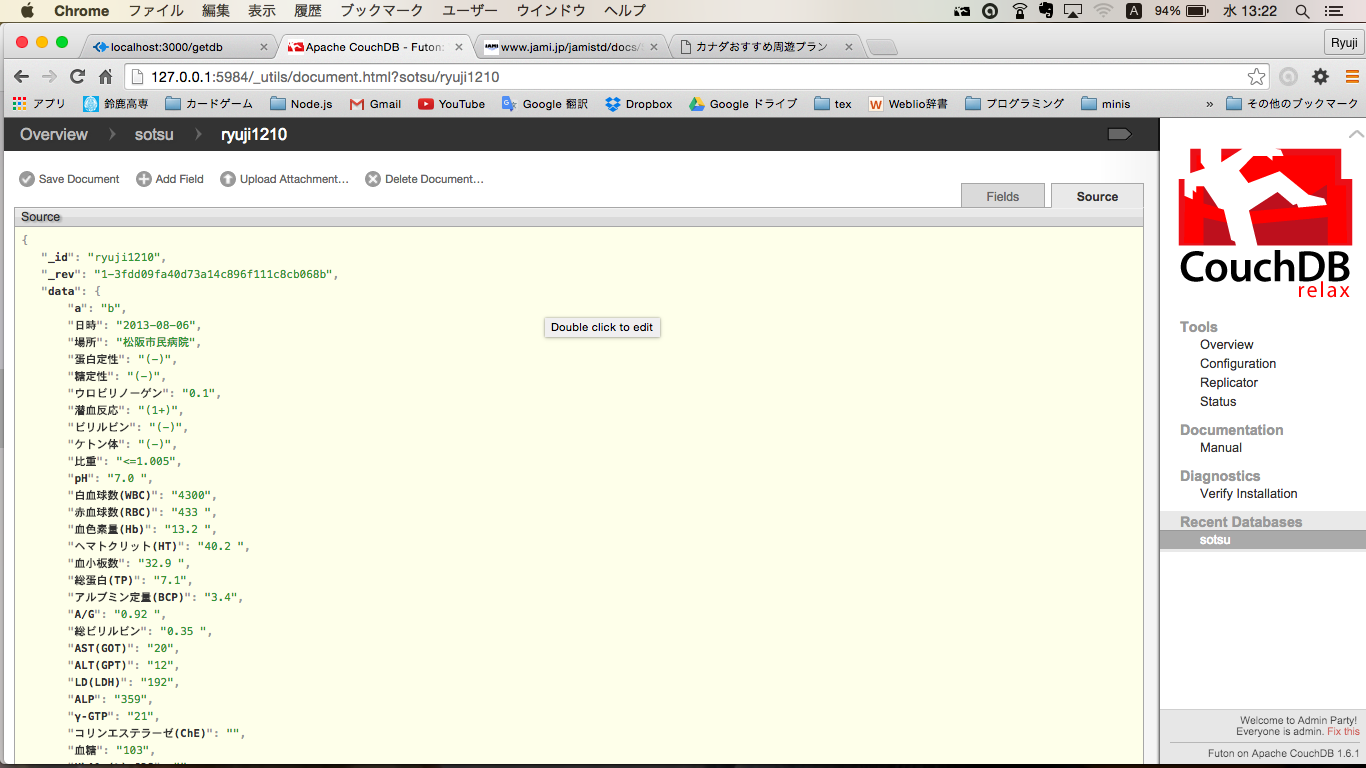
\includegraphics[width=5cm, bb=0 0 437 688]{./gazou/kensa.png}
				%\end{center}
				\caption{医療大の検査データ}
				\label{ss-mix_sampledata}
			\end{figure}

		\subsubsection{横向きcsvファイルの場合}
			holizontialparse
			医療大の投薬データ
			\\
			\begin{figure}[htbp]
				%\begin{center}
					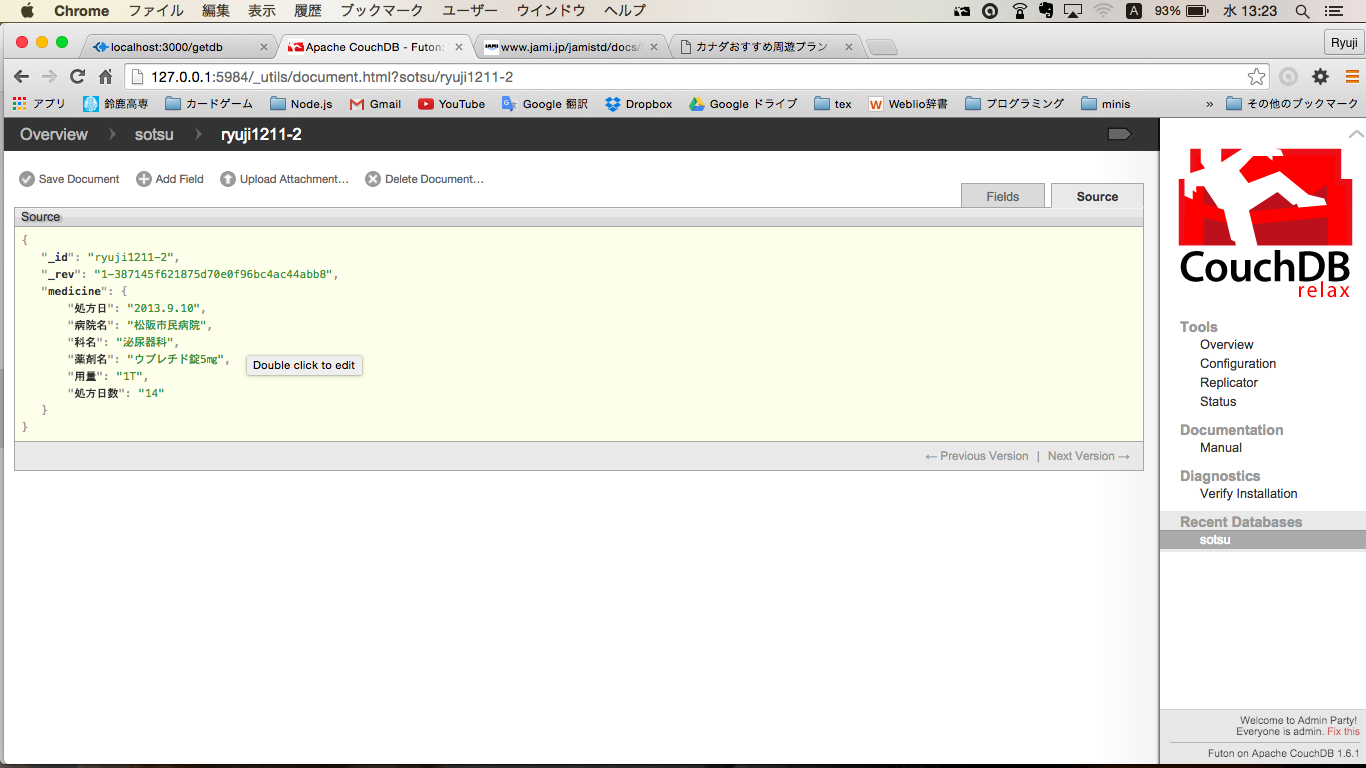
\includegraphics[width=5cm, bb=0 0 437 688]{./gazou/touyaku.png}
				%\end{center}
				\caption{医療大の投薬データ}
				\label{ss-mix_sampledata}
			\end{figure}

		\subsubsection{パイプ区切りのHL7ファイルの場合}
			parsehl7
			HL7のデータ
			\\
			\begin{figure}[htbp]
				%\begin{center}
					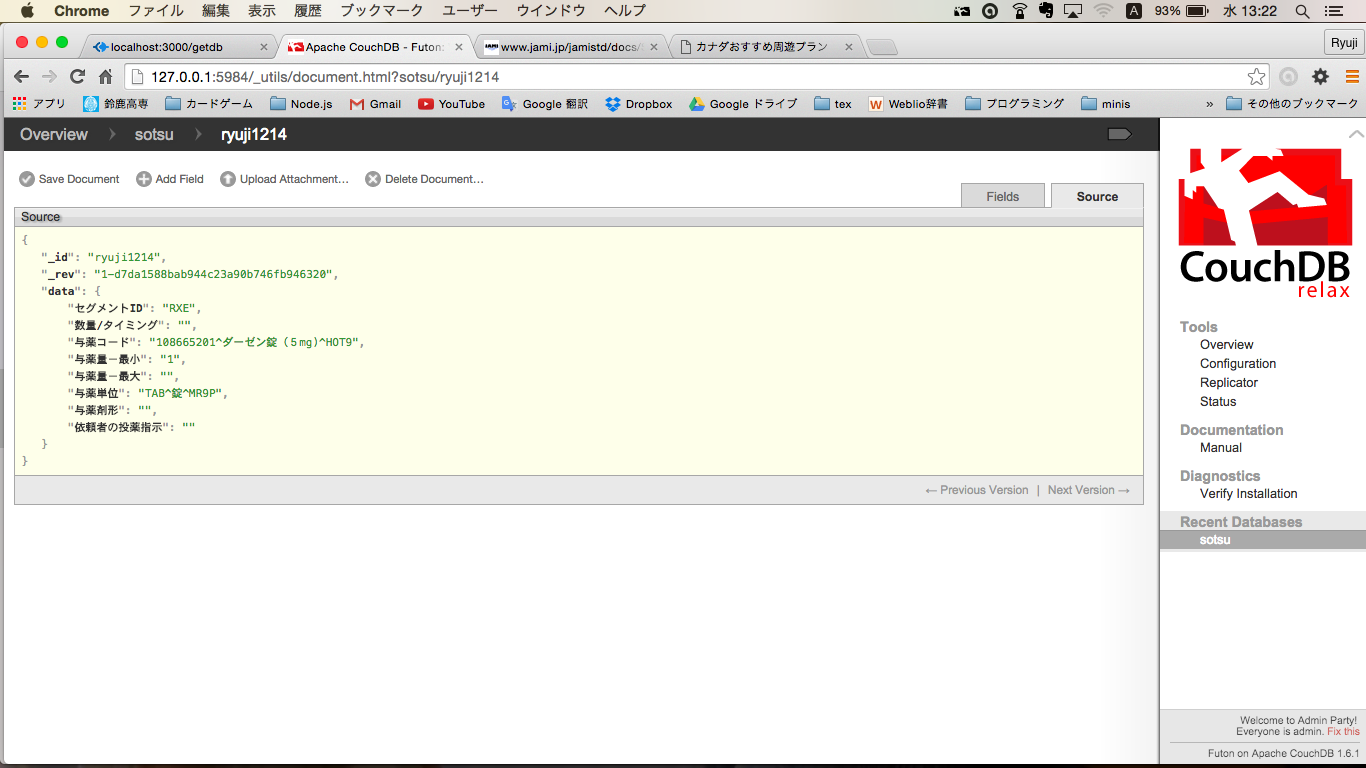
\includegraphics[width=5cm, bb=0 0 437 688]{./gazou/hl7.png}
				%\end{center}
				\caption{HL7のサンプルデータ}
				\label{ss-mix_sampledata}
			\end{figure}

			患者,医療関係者からの投入を受け付ける.
			ファイルを指定してpostで送信してる.


\subsection{同義キーの登録}
	\begin{figure}[htbp]
		%\begin{center}
			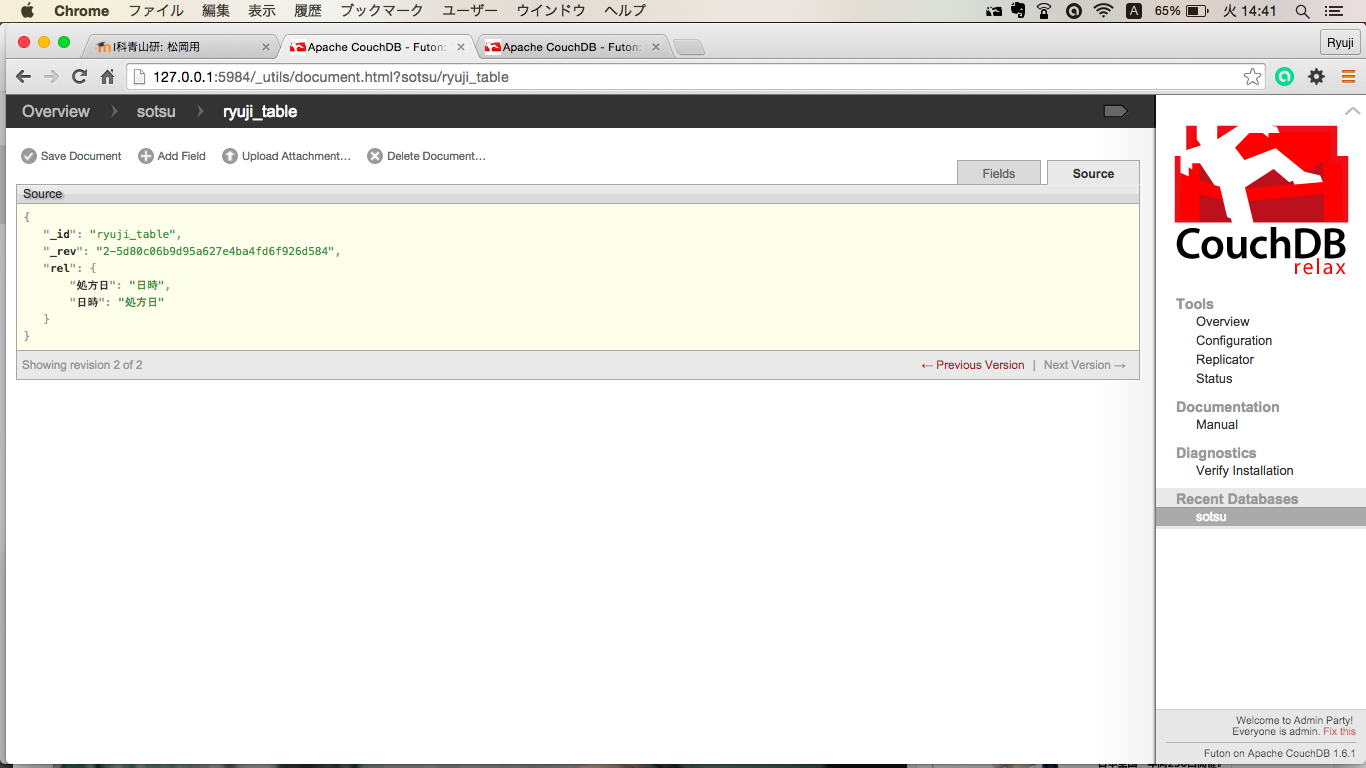
\includegraphics[width=5cm, bb=0 0 437 688]{./gazou/relation.png}
		%\end{center}
		\caption{同義キーを管理するドキュメント}
		\label{relation}
	\end{figure}

	\begin{figure}[htbp]
		%\begin{center}
			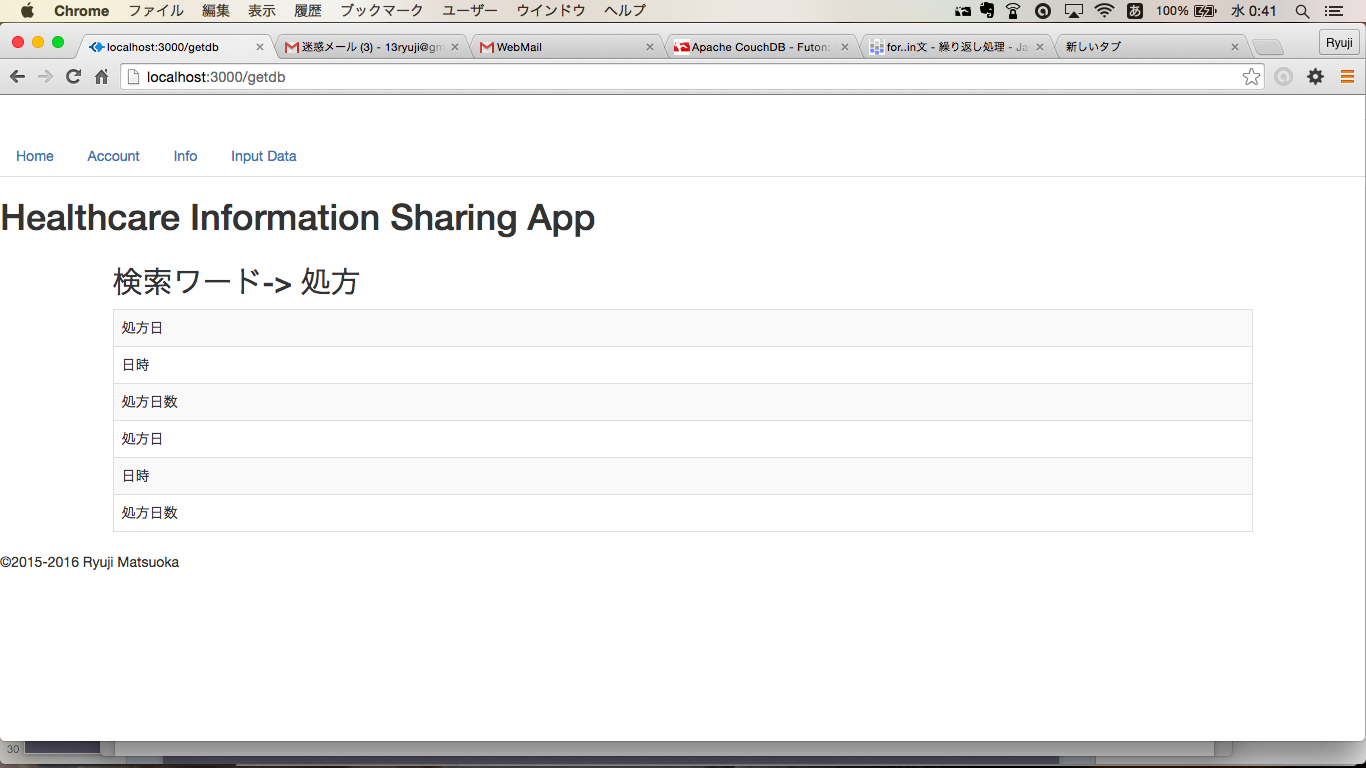
\includegraphics[width=5cm, bb=0 0 437 688]{./gazou/relationApp.png}
		%\end{center}
		\caption{処方と検索して同義キーとして登録されている日時を表示する}
		\label{relationApp}
	\end{figure}
